\documentclass[10pt,letterpaper,bibliography=totocnumbered]{scrartcl}

\usepackage[letterpaper,margin=1.2in]{geometry}
\usepackage{helvet}
\usepackage{graphicx}
\usepackage[hyphens]{url}
\usepackage{hyperref}
\usepackage[all]{hypcap} 
\usepackage{xcolor}
\usepackage{listings}
\usepackage[T1]{fontenc}
\usepackage{verbatim}
\usepackage{mathtools}
\usepackage{float}
\usepackage{csquotes}

\lstset{
    basicstyle=\scriptsize,
    numbers=left,
    numberstyle=\scriptsize,
    stepnumber=1,
    numbersep=5pt,
    showspaces=false,
    showstringspaces=false,
    showtabs=false,
    frame=shadowbox,
    tabsize=4,
    captionpos=b,
    breaklines=true,
    breakatwhitespace=false,
    keywordstyle=\color{blue!70},
    commentstyle=\color{red!50!green!50!blue!50},
    rulesepcolor=\color{red!20!green!20!blue!20},
    numberbychapter=false,
    stringstyle=\ttfamily
}

\setcounter{tocdepth}{2}

\hypersetup{
    colorlinks=true,
    breaklinks=true,
    urlcolor=blue,
    linkcolor=black
}

\begin{document}

\author{Mathew Chaney}
\title{Assignment 4}
\subtitle{Fall 2016\\ CS834 Introduction to Information Retrieval\\ Dr. Michael Nelson}
\maketitle
\newpage

\tableofcontents
\listoffigures
\listoftables

\section{Question 10.5}

\subsection{Question}
Find a community-based question answering site on the Web and ask two
questions, one that is low-quality and one that is high-quality. Describe the answer quality of each question.

\subsection{Approach}
Yahoo! Answers is the question and answering website I chose to answer this question.  First, the high quality question I asked was ``How is the probability of precipitation calculated by meteorologists?''.  

I deem this question to be of high quality based on grammaticality, spelling and punctuation, as well as the use of concise terminology that may be slightly obscure to an uneducated reader.

It is also a focused question that has a definite set of answers.  There are a finite number of ways to perform the calculation in question, and they are well known.  The ideal answerer is even included as part of the question.  Refer to Table \ref{tab:goodq} to see some example answers for this question.


\begin{table}[H]
\centering
\begin{tabular}{ c }
Question: How is the probability of precipitation calculated by meteorologists?\\
\hline\hline
Trump is Putin's *****\\
\hline
Ye\\
\hline
we got hakerzed in the ***\\
\hline
no\\
\hline
Penis\\
\hline
\end{tabular}
\caption{Question and responses of good quality.}
\label{tab:goodq}
\end{table}


For the poor quality question I asked ``Trump is not russia, y u no belief he got hakerz to do it to us?''.  It begins with a premise that doesn't make sense, even the most uneducated person wouldn't suspect that Trump \textit{is} Russia.  It also lacks focus as to what is being asked or and has no real context and is full of misspellings and terrible grammar.  Correspondingly, the answers were lacking content, using poor grammar and exhibiting numerous spelling errors, and some possibly offensive to some readers.  Refer to Table \ref{tab:badq} for the question again with some sample answers.


\begin{table}[H]
\centering
\begin{tabular}{ c }
Question: Trump is not russia, y u no belief he got hakerz to do it to us?\\
\hline\hline
Trump is Putin's *****\\
\hline
Ye\\
\hline
we got hakerzed in the ***\\
\hline
no\\
\hline
Penis\\
\hline
\end{tabular}
\caption{Question and responses of poor quality.}
\label{tab:badq}
\end{table}

\section{Question 10.6}

\subsection{Question}
Find two examples of document filtering systems on the Web. How do they build a profile for your information need? Is the system static or adaptive?

\subsection{Answer}
The first example I found was \url{www.amazon.com}.  This is an Internet marketplace where nearly any type of product can be purchased online and delivered to one's home.  The document filtering Amazon performs is done in an adaptive manner using a combination of the user data from previous purchases to recommend new items the user may be interested in.  The system can also recommend items that similar users often purchase that are also similar to items the user is viewing while browsing the item repository.  For example, if one purchases a mechanical pencil it is likely that the user will also be interested in purchasing graphite refill packages or extra replacement erasers.  This system changes over time as the database of related items is based on the past purchases of the different items and how some items are more often purchased together than others.



\section{Question 11.2}

\subsection{Question}
Does your favorite web search engine use a bag of words representation?  How can you tell whether it does or doesn't?

\subsection{Answer}
My favorite search engine is Google.  I am fairly certain they do not use the bag-of-words model described by the text book.

As an example, there is a well known online meme, or trend, called "y u no guy".  It is an image macro used to bring attention to something and uses a popular practice from online forums of shortening words to a single letter corresponding to the phonetic pronunciation of the word, e.g. ``you'' becomes ``u''.  The target message is accompanied by a cartoon man with a face of frustration and rage.  See Figure \ref{fig:yuno} for the results of issuing the query ``y u no'' to Google's search engine.

\begin{figure}[H]
\centering
\label{fig:yuno}
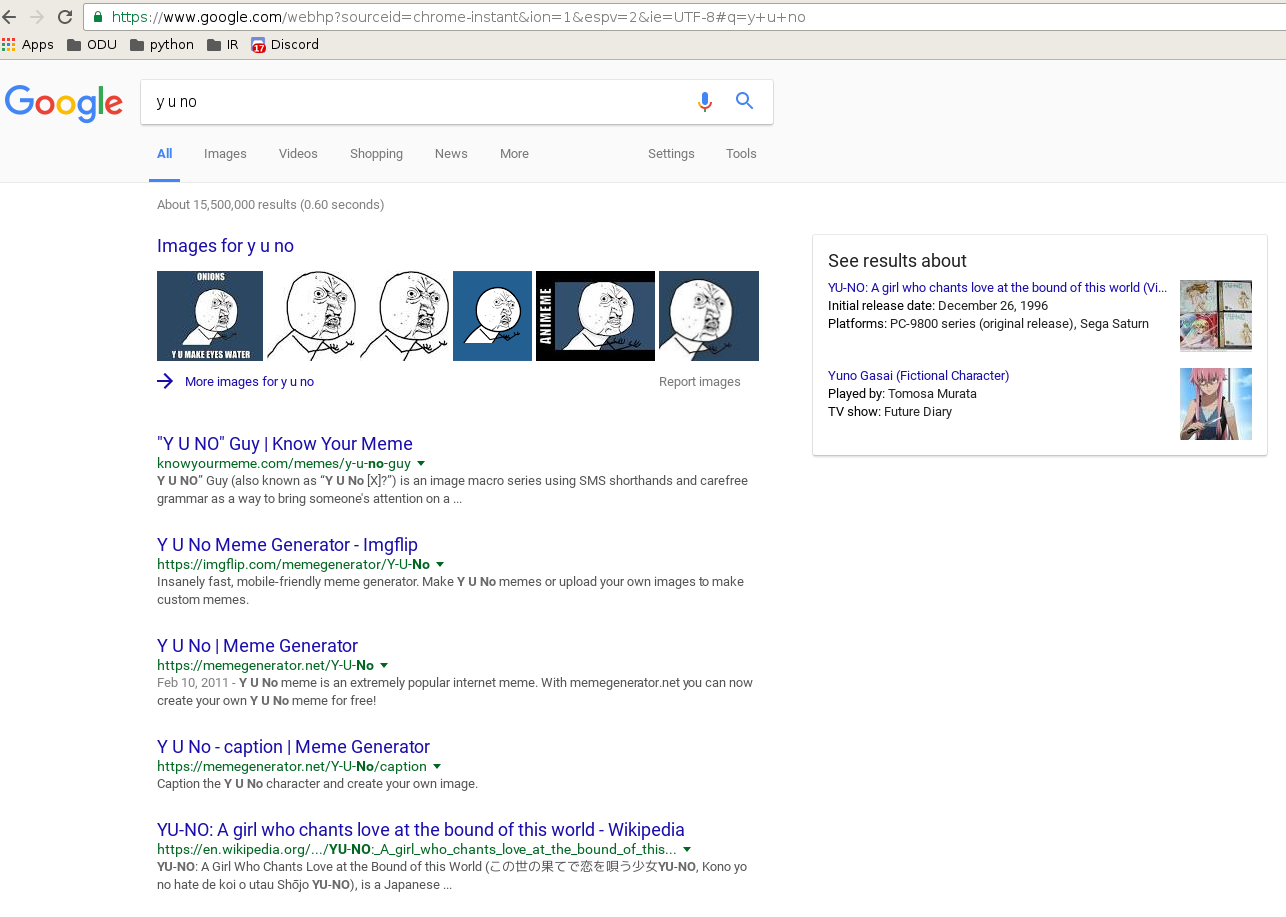
\includegraphics[scale=.35]{q11.2/yuno.png}
\caption{Google results from issuing the query ``y u no''}
\end{figure}

Google recognizes these three simple terms to be part of a phrase and retrieves results based on that phrase with a high degree of accuracy.

\clearpage

To show that Google's engine does not use the bag-of-words model, consider this similar search with the terms ``no u y''.

\begin{figure}[H]
\centering
\label{fig:nouy}
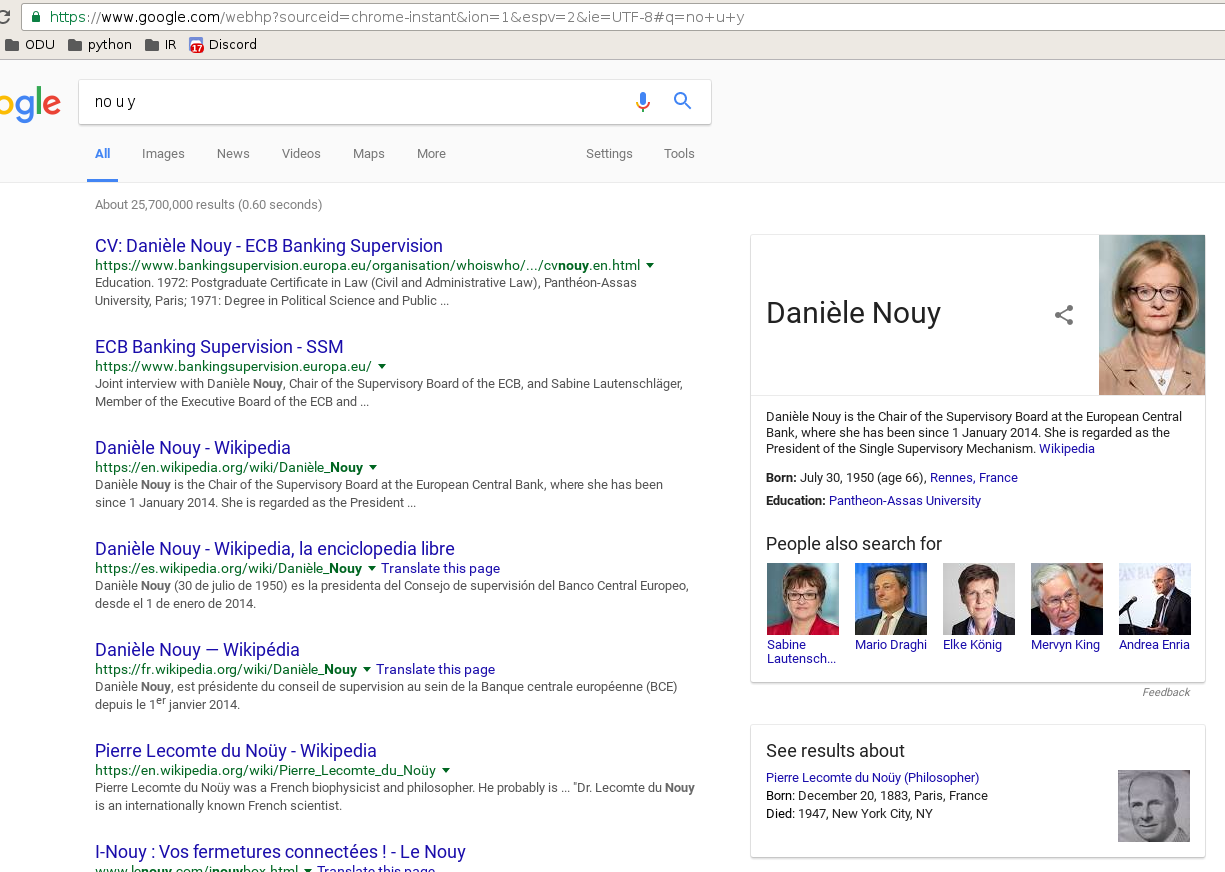
\includegraphics[scale=.35]{q11.2/nouy.png}
\caption{Google results from issuing the query ``no u y''}
\end{figure}

With the same three terms in a different order, a completely different ranking is presented by the search engine.  The results for this search are not regarding y u no guy at all, they are dominated by pages about the Chair of the Supervisory Board at the European Central Bank, Daniele Nouy.  This shows that Google's engine accounts for query term ordering, which would not be present in a plain bag-of-words retrieval model.

\section{Question 11.4}

\subsection{Question}
Show how the linear feature-based ranking function is related to the abstract ranking model from Chapter 5.


\subsection{Answer}
Starting with the first mention of the abstract ranking model, refer to Figure \ref{fig:51}.  This is an example of the ranking function for a single document.

\begin{figure}[H]
\centering
\label{fig:51}
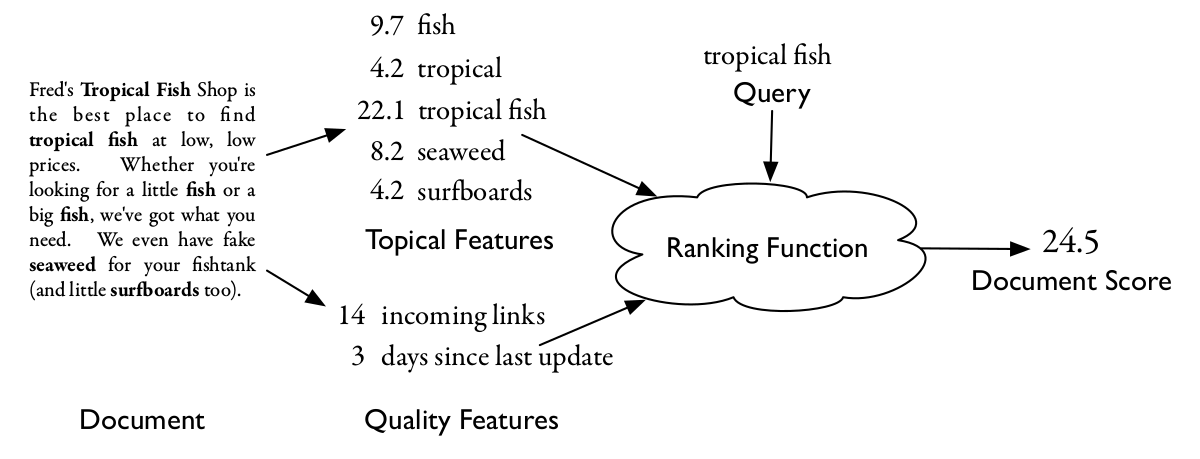
\includegraphics[scale=.25]{q11.4/fig51.png}
\caption{The components of the abstract model of ranking\dots}
\end{figure}

And a more formal definition of the abstract ranking model can be found in equation \ref{eq:1}:

\begin{equation}
\label{eq:1}
R(Q, D) = \sum_i g_i (Q) f_i (D)
\end{equation}

This is a linear combination of two feature functions, \(f_i\) is a feature function that extracts a score from the document and \(g_i\) is a feature function that extracts a score from the query.\\

Now, for a definition of the linear feature-based retrieval model, refer to Equation \ref{eq:2}:

\begin{equation}
\label{eq:2}
S_\Lambda(D;Q) = \sum_j \lambda_j \cdot f_j(D, Q) + Z
\end{equation}

here, \(f_j\) is a feature function that maps query/document pairs to real values, i.e. scores, so it is also a linear combination of functions that emit scores based on features of some related piece of the components of the formulation, either the document, the query, some parameter (\(\lambda \in \Lambda\)), or a constant that is not related to the document but could be related to the query (\(Z\)).  This is very similar to how the abstract ranking model functions in that it is a summation of a group of scoring functions over the elements to be ranked.  The mechanism is the same as before with the abstract model, with the addition of the \(\lambda\) parameters.

\section{SVM Light Example}

\subsection{Inductive Example}
SVM Light \cite{svmlight} and the Inductive example were downloaded from \url{http://www.cs.cornell.edu/People/tj/svm_light/}.\\

Following the instructions in the Inductive example, the \texttt{svm\_learn} program was invoked on the training data file train.dat, the output from which can be found in Listing \ref{listing:svmlearn}.  This produced the model file that is used in the classification step.

\lstinputlisting[language={}, caption={output of the svm\_learn program using the train.dat data file}, label=listing:svmlearn,linerange={1-27},firstnumber=1]{code/svmlight/svmlearn.txt}

After the model file was generated the example directs the user to run the \texttt{svm\_classify} program on the provided test data \texttt{(filename: test.dat)} using the training model \texttt{(filename: model)} from the previous step.  The output of this can be found in Listing \ref{listing:svmclass}.

\lstinputlisting[language={}, caption={output of the svm\_classify program using the model training data file}, label=listing:svmclass,linerange={28-35},firstnumber=28]{code/svmlight/svmlearn.txt}

\subsection{Discussion}
As the results show, the precision was 96.67\% and the recall was 99.00\%, which are very high scores for these measures.  


\bibliography{report}
\bibliographystyle{unsrt}

\end{document}
